\chapter{物理信息-生成式正逆向流变学本构建模研究}
% 引言 引出第四章内容
\section{引言}
流变学本构建模长期面临实验数据与理论模型间的鸿沟。传统方法常基于理想化假设构建本构方程,虽能获得形式优美的数学模型,却难以准确表征真实材料在复杂工况下的非线性响应。基于前章通过PI-GRU网络对流变数据的时序建模基础,本章则提出物理信息驱动与生成式建模融合的新范式,通过融合频率域的真实实验数据与物理守恒定律的强约束机制,构建兼具高预测精度与可定制性的智能建模框架。

当前流变学本构建模领域存在两大核心问题,第一个问题是传统物理模型在描述真实材料复杂流变行为时,常因过度简化导致预测偏差累积,而纯数据驱动的黑箱模型虽能实现高精度拟合,却丧失了物理可解释性这一流变学研究的本质诉求,同时由于流变学数据往往依赖于各类流变仪的实验测量,所以优质的流变学数据是稀有的,本文前一章使用数值模拟方法可以生成大量模拟数据,但是这在真实实验上不可以复刻。Mahmoudabadbozchelou提出的一类PINN方法,通过多保真建模,首先通过对实验数据进行本构方程的参数拟合,然后借用拟合后的方程进行数值模拟生成大量低保真数据,之后使用高保真数据(原本的实验数据)和低保真数据(模拟数据)联合进行深度学习训练,在一定程度上缓解了数据不足问题,同时由于低保真数据本身是符合经典本构方程的,具有一定物理约束意义。本章参考了Mahmoudabadbozchelou的方法,来对一类黏弹性聚合物凝胶的流变学数据:储存模量(G')、损耗模量(G")和损耗角正切(tan$\delta$)进行PINN建模,尝试构建材料制备参数、频率到流变学性质的模型映射。在Mahmoudabadbozchelou的基础模型中,本文引入了几个优化,首先是通过引入可学习的损失函数权重,使得模型在训练过程中,能够根据训练数据中不同参数的分布情况,动态调整损失函数的权重,从而提高模型泛化能力,其次在特征工程方面,引入注意力特征融合的方法,进一步解决实验数据特征稀疏的问题。

第二个问题是材料逆向设计过程中,基于试错法的实验优化模式耗费大量资源,而现有生成模型在流变学参数空间的可控生成方面缺乏物理约束,导致生成结果常偏离热力学可行域。近年来,许多研究者聚焦于材料制备参数到流变学性质的建模,但是实际应用中,根据已知的期望的材料性质,通过反向建模来确定这种材料应该如何制备也是非常重要。考虑到多组分材料体系的流变指纹具有高维参数空间中的低维流形特性,变分自编码器(VAE)的潜空间建模应用于流变学的反向建模是可行的,本章使用了VAE类模型中的条件变分自编码器(CVAE)来进行反向建模,探究特定制备参数到流变学特性的可控映射。

本章创新性地将物理信息神经网络(PINN)与条件变分自编码器(CVAE)进行耦合,建立双向建模通道:在正向建模路径中,通过将已知的本构方程编码为PINN的软约束条件,有效解决了小样本实验数据下的过拟合问题;在逆向设计路径中,利用CVAE的潜空间探索能力,结合流变响应的物理可行性验证模块,实现了从目标流变特性到材料制备参数的可控映射。这种混合建模策略不仅突破了传统方法在数据-物理融合层面的技术壁垒,更重要的是构建了闭环的材料设计-验证工作流,为智能流变学提供一定方法论基础。
% 实验设计  描述本章的实验过程,介绍黄金的工作,模型相关公式等等
\section{实验设计}
\subsection{PINN-CVAE正逆向建模架构}
\begin{figure}[htbp]
  \centering
  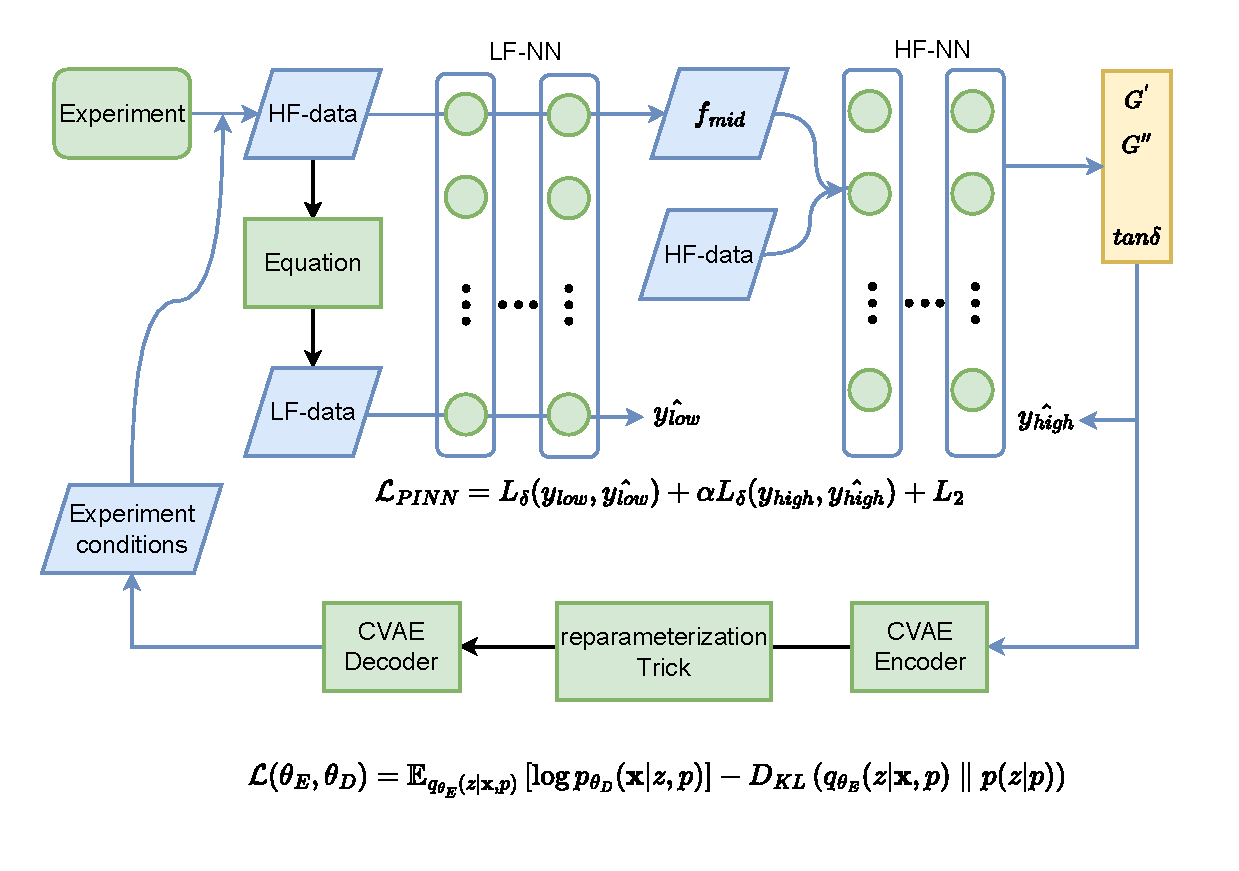
\includegraphics[width=0.8\textwidth]{Fig/PINN-CVAE.pdf}
  \FigureBicaption{\label{PINN-CVAE-illustration}PINN-CVAE正逆向建模架构}{Schematic illustration of the PINN-CVAE model}
\end{figure}


\subsection{PINN数据预处理}
\subsubsection{实验数据来源}
本章所有训练和测试的实验数据是基于Huang等人的工作\cite{huangUltrahighEnergydissipationElastomers2021}。Huang等人介绍了一种将粘性聚合物流体(PBA)注入弹性网络中,形成聚合物流体凝胶(PFGs),以实现宽频带可控超高能量耗散的策略,如图\ref{huangjin-illustration}所示。
\begin{figure}[htbp]
  \centering
  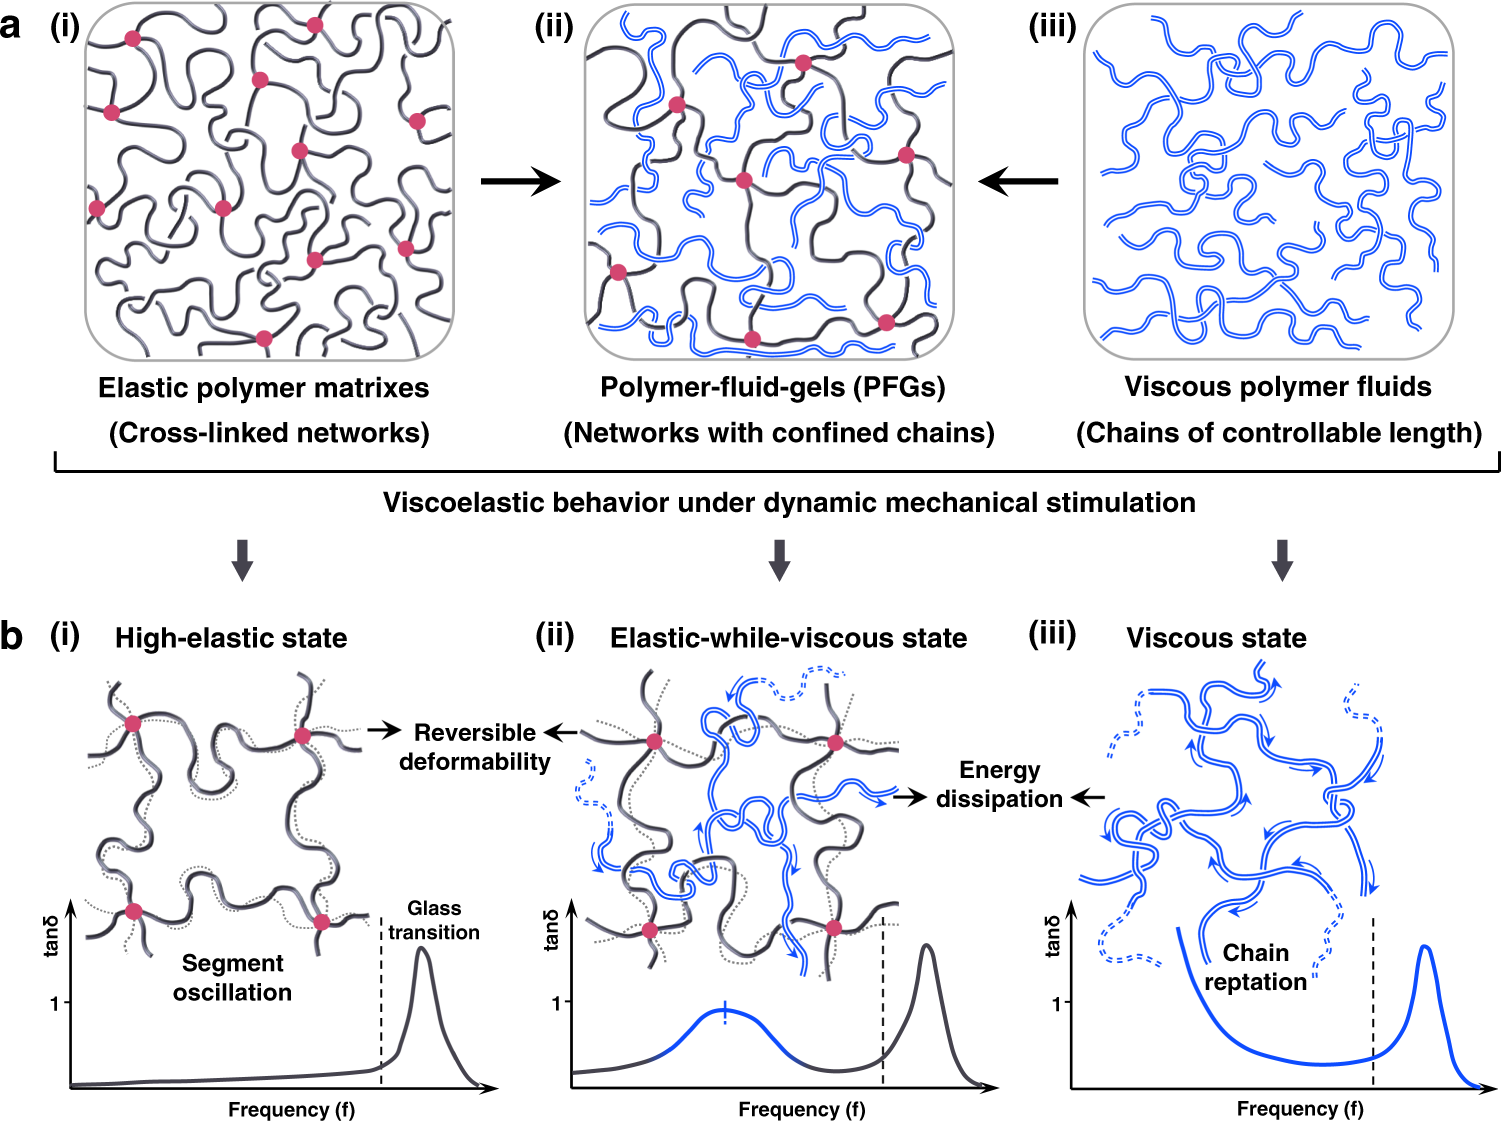
\includegraphics[width=0.8\textwidth]{Fig/huangjin.png}
  \FigureBicaption{\label{huangjin-illustration}Huang等人制备的PFGs示意图}{Schematic illustration of the PFGs prepared by Huang et al.}
\end{figure}
在实验过程中,Huang等人对不同分子量的PBA流体,注入不同分子量PBA制备的PFGs,分别进行了流变学实验,得到了对应材料特定频率下的储存模量、损耗模量和损耗角正切等数据。本章采用他们的实验数据进行具体的深度学习建模。

\subsubsection{实验数据分类}
首先本节对真实实验数据进行分类,第一类为单PBA流体数据,为不同分子量的PBA流体的流变学数据,特征包括:聚合度(DP)、数均分子量(Mn)、分散指数(PDI)、频率($\omega$),标签包括:储存模量(G')、损耗模量(G")和损耗角正切(tan$\delta$),第二类为单分子量PBA注入制备的PFGs数据,特征和标签和第一类单PBA流体数据一致,第三类为多分子量PBA注入制备的PFGs数据,特征包括:不同分子量的PBA特征和组分信息(Mn$_i$、PDI$_i$、DP$_i$、$\phi_i$,$i=1,2,3$)、频率($\omega$),标签包括:储存模量(G')、损耗模量(G")和损耗角正切(tan$\delta$)。第三类数据的组分信息见表\ref{pba-com-groups}所示。
\begin{table}
  \TableBicaption{\label{pba-com-groups}多分子量PBA流体制备PFGs的配比参数表}{Formulation Parameters of Multi-MW PBA Fluids for PFGs}
  \centering
  \small
  \begin{tabularx}{\textwidth}{>{\centering\arraybackslash}X >{\centering\arraybackslash}X} % 关键修改点
    \Xhline{1.5pt}
    实验分组   & \makecell{
      \begin{tabular}{@{}c@{}}
        $\phi_{PBA}(\%)$ \\
        \Xhline{0.5pt}
        Mn(20k,35k,52k,78k,102k,152k)
      \end{tabular}
    }                         \\
    \Xhline{0.5pt}
    PFG-b1 & (0,20,0,0,30,10) \\
    PFG-b2 & (0,30,0,30,0,0)  \\
    PFG-b3 & (20,0,0,40,0,0)  \\
    PFG-b4 & (10,0,20,30,0,0) \\
    PFG-b5 & (0,0,30,0,0,30)  \\
    PFG-b6 & (0,0,20,0,0,40)  \\
    \Xhline{1.5pt}
  \end{tabularx}
\end{table}
\subsubsection{低保真数据生成}
分类后,本节使用Doi-Edwards模型来进行低保真数据拟合。首先假设实验数据可以使用Doi-Edwards模型描述。Doi-Edwards模型的频率域公式可以通过时间域公式进行傅里叶变换得到公式\eqref{eq:doi-edwards-g1}和公式\eqref{eq:doi-edwards-g2}
\begin{align}
  G'(\omega) = G_0 \frac{8}{\pi^2} \sum_{p=1,3,5,\ldots}^{\infty} \frac{1}{p^2} \frac{1}{1 + (\omega \tau_d / p^2)^2} \label{eq:doi-edwards-g1} \\
  G''(\omega) = G_0 \frac{8}{\pi^2} \sum_{p=1,3,5,\ldots}^{\infty} \frac{1}{p^2} \frac{\omega \tau_d / p^2}{1 + (\omega \tau_d / p^2)^2}
  \label{eq:doi-edwards-g2}
\end{align}
本节使用Python的scipy.optimize库对真实数据进行最小二乘法的拟合,为了简化运算设置公式中的$p$为1,得到Doi-Edwards模型的拟合参数。之后根据拟合后的方程,通过Numpy库生成频率-模量数据,用于后续的PINN模型训练,这一部分数据被称为低保真数据(LF-data)。

\subsubsection{数据集划分}
本节将数据集划分为训练集、验证集和测试集,其中训练集和验证集用于模型训练,测试集用于模型验证。对于PBA流体数据取DP值为162的数据为测试集,其余数据为训练集和验证集,训练集和验证集按照9:1的比例划分。对于单分子量PBA注入制备的PFGs数据,取DP值为162的数据为测试集,其余数据为训练集和验证集,训练集和验证集按照9:1的比例划分。对于多分子量PBA注入制备的PFGs数据,取PFG-b2组(分组见表\ref{pba-com-groups})的数据为测试集,其余数据为训练集和验证集,训练集和验证集按照9:1的比例划分。

% 模型训练细节
\subsection{PINN模型训练}
\subsubsection{损失函数构建}
本节使用PINN模型对低保真数据(LF-data)和高保真数据(HF-data)进行训练。模型架构包含两个多层感知机(MLP)网络:低保真网络$\mathbf{M_{low}}$和高保真网络$\mathbf{M_{high}}$。训练流程如下:

首先低保真数据$X_{low}$首先通过低保真网络得到预测值$\hat{y}_{low}$,与真实低保真标签$y_{low}$计算物理损失。之后高保真数据$X_{high}$通过低保真网络得到中间特征$f_{mid}$,将$f_{mid}$与$X_{high}$拼接后输入高保真网络,得到最终预测值$\hat{y}_{high}$。$\hat{y}_{high}$与真实高保真标签$y_{high}$计算数据损失,并与物理损失拼接得到总损失。

具体计算过程可表示为公式\eqref{eq:lf-model}和公式\eqref{eq:hf-model}:
\begin{align}
  \hat{y}_{low}  & = \mathbf{M_{low}}(X_{low}) \label{eq:lf-model}                               \\
  \hat{y}_{high} & = \mathbf{M_{high}}(X_{high}, \mathbf{M_{low}}(X_{high})) \label{eq:hf-model}
\end{align}

本节使用Python语言和PyTorch深度学习框架实现模型训练。在优化策略方面,采用Adam优化器进行参数更新,并引入基于性能指标的学习率调度机制实现自适应学习率调整。为获得最优的模型结构,本文结合网格搜索和随机搜索两种方法对关键超参数进行系统调优,包括网络层数、每层神经元数量、初始学习率、正则化强度、训练轮次以及批次大小等。

在损失函数选择上,考虑到实验数据中可能存在的异常值和噪声,本文采用鲁棒性较好的Huber损失函数,其定义如公式\eqref{eq:huber-loss}所示:
\begin{equation}
  \begin{aligned}
    L_\delta(y, \hat{y}) =
    \begin{cases}
      \frac{1}{2}(y - \hat{y})^2                 & \text{if } |y - \hat{y}| \le \delta    \\
      \delta |y - \hat{y}| - \frac{1}{2}\delta^2 & \text{otherwise} \label{eq:huber-loss}
    \end{cases}
  \end{aligned}
\end{equation}
Huber损失函数通过参数$\delta$实现对异常值敏感度的动态调节:当$\delta$趋近于0时,其行为接近平均绝对误差(MAE),表现出对异常值的强鲁棒性;当$\delta$较大时,其特性近似于均方误差(MSE),保持了较高的训练效率。这种自适应特性使得模型能够在保持训练稳定性的同时,有效应对实验数据中的噪声干扰。

本节在基本的PINN损失函数构建公式中添加可学习的权重$\alpha$,如公式\eqref{eq:pinn-loss-weight},通过权重$\alpha$平衡损失强度,适应不同的训练任务。
\begin{equation}
  L_{\text{PINN}} = \underbrace{L_\delta(y_{low}, \hat{y}_{low})}_{\text{低保真物理损失}} + \alpha \cdot \underbrace{L_\delta(y_{high}, \hat{y}_{high})}_{\text{高保真数据损失}}  \label{eq:pinn-loss-weight}
\end{equation}

\subsubsection{特征融合细节}
本章中4.2.1中提到的的第一类和第二类数据的PINN训练均直接按照PINN方案进行训练,第三类数据涉及不同分子量的分子量和组分数据,在训练时分别采用哈达玛积特征融合和注意力特征融合的方法进行特征融合,再进行训练。哈达积融合方法如公式\eqref{eq:hadamard-product-Mn},
\begin{equation}
  \mathbf{Mn} \circ \mathbf{w} =
  \begin{bmatrix}
    M_{n_1} \cdot w_1 \\
    M_{n_2} \cdot w_2 \\
    \vdots            \\
    M_{n_k} \cdot w_k
  \end{bmatrix} \label{eq:hadamard-product-Mn}
\end{equation}
即将不同的分子量与其对应的组分进行哈达玛积融合,这有助于模型更好地理解特征间的关系,优化训练效果。该操作的本质是构建流变学特征基元,其中高分子链的松弛行为同时受$Mn$(链长)和$w_i$(浓度)调控。

公式\eqref{eq:Mn-w-hadamard-slice}表示经过哈达玛积融合后的结果,根据$\mathbf{H}$按照公式\eqref{eq:Attention-Q}到\eqref{eq:Attention-V}计算$\mathbf{Q}$、$\mathbf{K}$和$\mathbf{V}$。$\mathbf{Q}$(Query)是编码目标流变性能的特征查询,$\mathbf{K}$(Key)表征各组分分子量分布的"响应指纹",$\mathbf{V}$(Value)携带原始流变特征的实际物理量级信息。

\begin{equation}
  \mathbf{H} =
  \begin{bmatrix}
    Mn_{1} \cdot w_1 \\
    Mn_{2} \cdot w_2 \\
    Mn_{3} \cdot w_3
  \end{bmatrix} \label{eq:Mn-w-hadamard-slice}
\end{equation}
\begin{align}
  \mathbf{Q} & = \mathbf{W}_q \mathbf{H}, \quad \mathbf{W}_q \in \mathbb{R}^{d \times 3}  \label{eq:Attention-Q} \\
  \mathbf{K} & = \mathbf{W}_k \mathbf{H}, \quad \mathbf{W}_k \in \mathbb{R}^{d \times 3} \label{eq:Attention-K}  \\
  \mathbf{V} & = \mathbf{W}_v \mathbf{H}, \quad \mathbf{W}_v \in \mathbb{R}^{d \times 3} \label{eq:Attention-V}
\end{align}
% 步骤3: 注意力分数计算
之后使用公式\eqref{eq:Attention-score}计算注意力分数,注意力分数量化了组分间的流变学相互作用,该机制可自动识别关键组分,例如高分子量组分($M_{n_1} > M_{n_2}$)对模量等的主导作用。
\begin{equation}
  \text{Attention}(\mathbf{Q}, \mathbf{K}, \mathbf{V}) = \text{softmax}\left(\frac{\mathbf{Q} \mathbf{K}^\top}{\sqrt{d}}\right) \mathbf{V} \label{eq:Attention-score}
\end{equation}
最后使用公式\eqref{eq:Attention-output}计算最终的注意力输出。
% 步骤4: 最终融合输出
\begin{equation}
  \mathbf{Z} = \text{LayerNorm}(\mathbf{H} + \text{Attention}(\mathbf{Q}, \mathbf{K}, \mathbf{V}))
  \label{eq:Attention-output}
\end{equation}

本节分别使用原始特征的PINN、哈达玛积特征融合后的PINN和注意力特征融合后的PINN训练多分子量PBA注入制备的PFGs数据,得到不同的训练模型。

\subsection{PINN模型测试}
本节对训练模型进行测试,并分析训练结果,对于第一类数据(单PBA流体数据)和第二类数据(单分子量PBA注入制备的 PFGs数据),使用DNN和PINN两种模型分别训练。保存模型后,使用测试数据进行预测,并分析预测结果。绘制真实值-预测值曲线,残差曲线进行定性分析。计算指标:决定系数R$^2$、平均绝对误差MAE、平均百分比误差MAPE和训练时间Training Time,并绘制指标对比图进行定量分析。

对于第三类数据(多分子量 PBA 注入制备的 PFGs 数据),本节分别使用DNN、PINN、哈达玛积特征融合后的PINN和注意力特征融合后的PINN进行训练,对不同的训练模型进行测试,并分析训练结果,具体分析方法同上。

\subsection{CVAE反向建模训练}
本节使用条件变分自编码器(CVAE)进行反向建模,将PFG-b4的数据作为测试集,其余数据为训练集和验证集,训练集和验证集按照9:1划分,输入特征改为[$\omega$、G'、G"、tan$\delta$]序列,输出标签为制备参数:$M_{n_i}$和$w_i$。

本节使用Python的Pytorch库编写CVAE代码,并使用训练数据进行训练,得到模型参数。CVAE的损失函数公式如公式\eqref{eq:cvae-expriment}所示,其中$x = [w, G', G'', \tan \delta]$,$p = { M_{n_i}, w_i }'$。
\begin{equation}
  \mathcal{L}(\theta_E, \theta_D) = \mathbb{E}{q{\theta_E}(z|\mathbf{x},p)} \left[ \log p_{\theta_D}(\mathbf{x}|z,p) \right] - D_{KL}\left(q_{\theta_E}(z|\mathbf{x},p) | p(z|p)\right) \label{eq:cvae-expriment}
\end{equation}
CVAE的训练模型采用Adam优化器来进行优化,采用余弦退火算法自动调整学习率,采用网格搜索算法和随机搜索算法对超参数进行调优,其中超参数包括:隐藏层数、隐藏层节点数、学习率、迭代次数、批次大小,隐藏层激活函数采用ReLU6激活函数。
\subsection{CVAE反向建模测试}
本节通过CVAE训练频率-模量序列到组分信息的映射,将训练好后的模型保存。生成测试数据时,首先加载保存的模型参数,并输入目标制备条件$p = { M_{n_i}, w_i }'$作为生成约束;随后从条件先验分布$p(z∣p)$中采样潜在变量$z$(通过重参数化技巧$z=\mu_p+\epsilon⋅\sigma_p$实现可导性,其中$\epsilon$服从标准正态分布),将其与条件变量$p$拼接后输入解码器网络$p_{\theta_D}(\mathbf{x}|z,p)$,生成对应的$x = [w, G', G'', \tan \delta]$。为增强生成多样性,通过潜在空间插值或对条件参数p施加微小扰动生成100个多模态解。

针对生成的多模态解,本节通过多模态分布分析揭示其内在结构特征,采用核密度估计与箱线图结合的小提琴图可视化方法,呈现不同模态下解的密度分布、峰值位置及离散程度。使用残差分析对预测值与理论解的偏离模式进行系统性检验。使用真实数据误差分析,采用平均绝对百分比误差(MAPE)量化多模态解的整体预测精度。

\subsection{正逆向联合建模}
本节将训练好的PINN模型和CVAE模型进行正逆向联合建模,将CVAE生成的组分信息作为PINN模型的输入的特征,验证CVAE生成的数据对最终的流变学性质参数的预测效果,并分析CVAE生成的数据对PINN模型预测效果的提升作用,绘制真实组分特征与CVAE生成的数据输入PINN模型后预测的流变学性质参数的对比图,并计算MAPE指标,进行定量分析。

% 结果与讨论 全面的数据展开
\section{结果与讨论}
% 低保真数据拟合 数据展示
\subsection{低保真数据拟合}
\begin{figure}[htbp]
  \centering
  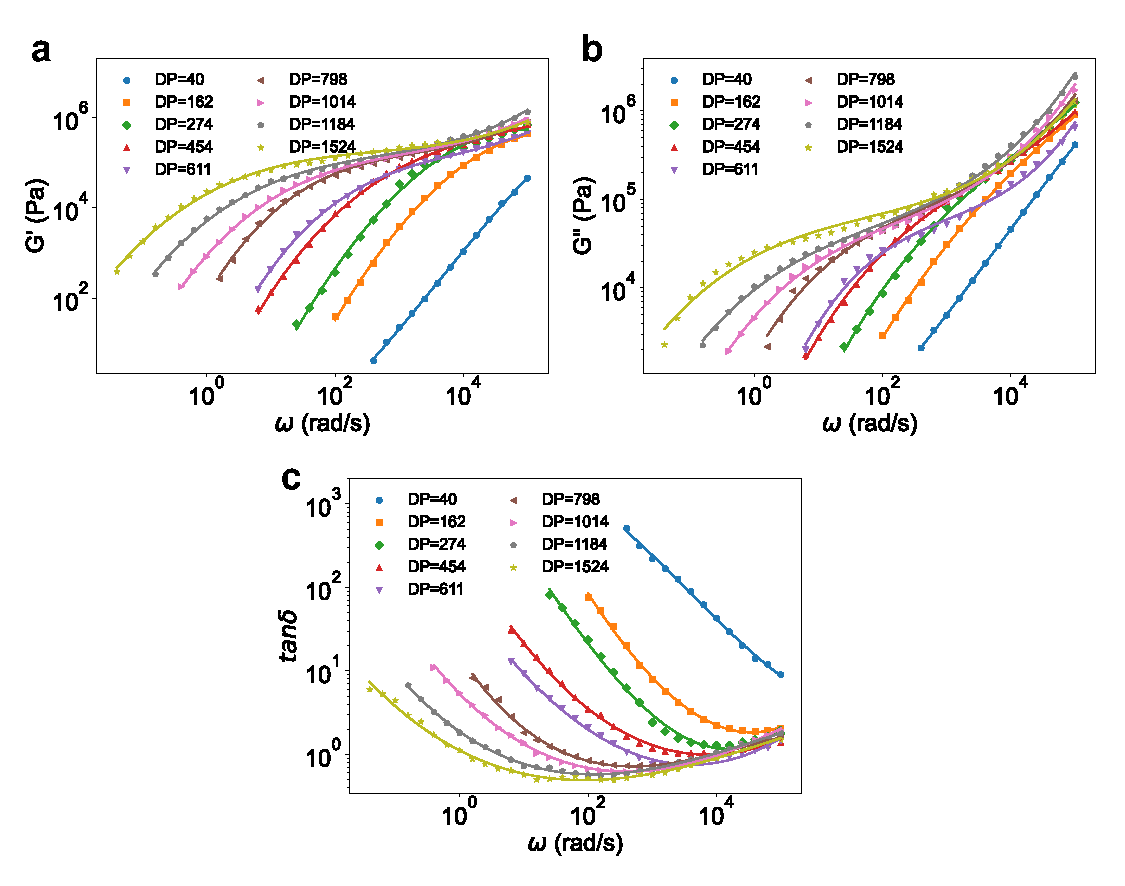
\includegraphics[width=0.8\textwidth]{Fig/pba-LF.pdf}
  \FigureBicaption{\label{pba-LF}不同PBA流体的频率-流变学性质参数数据低保真拟合结果:(a)不同DP值的PBA流体的频率-储存模量($\omega$-G')数据拟合结果;(b)不同DP值的PBA流体的频率-损耗模量($\omega$-G")数据拟合结果;(c)不同DP值的PBA流体的频率-损耗角正切($\omega$-tan$\delta$)数据拟合结果}{Low-fidelity fitting results of frequency-rheological property parameter data of different PBA fluids: (a) Fitting results of frequency-storage modulus ($\omega$-G') data of PBA fluids with different DP values; (b) Fitting results of frequency-loss modulus ($\omega$-G") data of PBA fluids with different DP values; (c) Fitting results of frequency-loss tangent ($\omega$-tan$\delta$) data of PBA fluids with different DP values}
\end{figure}
\begin{figure}[htbp]
  \centering
  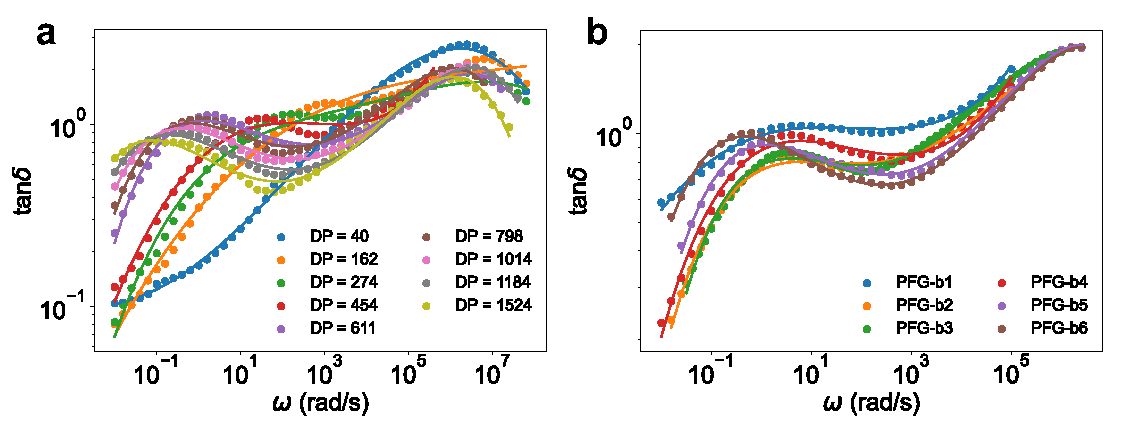
\includegraphics[width=0.8\textwidth]{Fig/pfgs-LF.pdf}
  \FigureBicaption{\label{pfgs-LF}}{不同PBA流体组合制备的PFGs的频率-流变学性质参数数据低保真拟合结果:(a)不同DP值的PBA流体制备的PFGs的频率-储存模量($\omega$-G')数据拟合结果;(b)不同PBA流体组合制备的PFGs的频率-损耗模量($\omega$-G")数据拟合结果;(c)不同PBA流体组合制备的PFGs的频率-损耗角正切($\omega$-tan$\delta$)数据拟合结果}{Low-fidelity fitting results of frequency-rheological property parameter data of PFGs prepared by different PBA fluid combinations: (a) Fitting results of frequency-storage modulus ($\omega$-G') data of PFGs prepared by PBA fluids with different DP values; (b) Fitting results of frequency-loss modulus ($\omega$-G") data of PFGs prepared by different PBA fluid combinations; (c) Fitting results of frequency-loss tangent ($\omega$-tan$\delta$) data of PFGs prepared by different PBA fluid combinations}
\end{figure}
本节使用Python的scipy.optimize库对真实数据进行最小二乘法拟合,既定函数为公式\eqref{eq:doi-edwards-g1}和\eqref{eq:doi-edwards-g2}。首先对PBA流体进行拟合,训练数据为不同聚合度(DP)的PBA流体的频率-储存模量($\omega$-G')数据、频率-损耗模量数据($\omega$-G")和频率-损耗角正切($\omega$-tan$\delta$)数据,拟合结果如图\ref{pba-LF}所示。从拟合曲线来看,不同PBA流体的拟合质量较优,拟合曲线和数据点贴合。表\ref{LF-metrics-table}展示了低保真数据的回归拟合指标,其中$g_1$、$g_2$、$g_3$分别对应不同PBA流体的$\omega$-G'、$\omega$-G"和$\omega$-tan$\delta$,可以看到这三组拟合指标的R$^2$指标都大于0.95,拟合效果优秀。
$g_1$组的MAPE值为19.72\%,$g_2$组的MAPE值为15.89\%,$g_3$组的MAPE值为12.45\%,根据统计学标准,MAPE值小于20\%被认为是可接受误差,这三组均在可接受范围,可以用于后续实验。
\begin{table}
  \TableBicaption{\label{LF-metrics-table}低保真数据拟合回归指标表}{Regression Metrics of Low-Fidelity Data Fitting}  % 中英文标题
  \centering
  \small
  \begin{tabularx}{\textwidth}{>{\centering\arraybackslash}X >{\centering\arraybackslash}X >{\centering\arraybackslash}X >{\centering\arraybackslash}X} % 关键修改点
    \Xhline{1.5pt}
    实验分组  & R$^2$   & MAE       & MAPE(\%)                \tabularnewline
    \Xhline{0.5pt}  % 表头下方线
    $g_1$ & $0.977$ & $456.78$  & $19.72$ \tabularnewline
    $g_2$ & $0.982$ & $2456.23$ & $15.89 $ \tabularnewline
    $g_3$ & $0.964$ & $5.17$    & $12.45$ \tabularnewline
    $g_4$ & $0.985$ & $0.25$    & $19.91$\tabularnewline
    $g_5$ & $0.962$ & $0.11$    & $9.89$\tabularnewline
    \Xhline{1.5pt}
  \end{tabularx}
\end{table}

之后,针对PBA流体注入制备的PFGs数据,使用最小二乘法进行拟合。图\ref{pfgs-LF}(a)展示了不同DP值的注入制备的PFGs数据的拟合曲线,拟合曲线和数据点贴合,拟合效果较优。图(a)对应的定量指标为表\ref{LF-metrics-table}的$g_4$,R$^2$值为0.985,MAPE值为19.91\%,均在可接受范围,可以用于后续实验。

图\ref{pfgs-LF}(b)展示了多分子量PBA注入制备的 PFGs 数据的拟合曲线,其中b1-b6是不同的PBA流体组合,具体组合如表\ref{pba-com-groups}所示。拟合曲线显示拟合效果优秀,定量指标如表\ref{LF-metrics-table}的$g_5$所示,R$^2$值为0.962,MAPE值为9.89\%,误差范围在可接受范围,可以用于后续实验。


% 单PBA流体本构建模
\subsection{单PBA流体本构建模}
本节首先对不同分子量的单PBA流体进行深度学习本构建模,分别建模预测储存模量(G')、损耗模量(G")和损耗角正切(tan$\delta$)。图\ref{pba-g1}为G'的预测结果,图\ref{pba-g1}(a)为真实-预测值曲线,从曲线图可以看到PINN建模的预测曲线相比DNN建模的预测曲线更为贴近真实数据点,拟合效果更佳。图\ref{pba-g1}(b)为残差图,PINN预测值与真实值的残差总体更为贴近0刻度线,极值范围相比DNN更小。根据图\ref{pba-g1},可以定性分析出PINN相比DNN在此项任务上具有更好的泛化预测效果。
\begin{figure}[htbp]
  \centering
  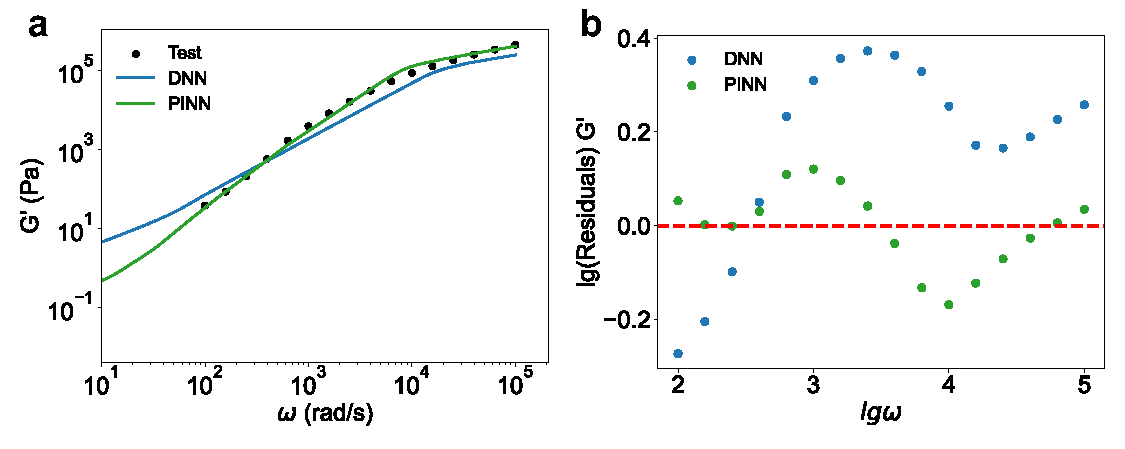
\includegraphics[width=0.8\textwidth]{Fig/pba-g1.pdf}
  \FigureBicaption{\label{pba-g1}不同分子量的PBA流体PINN和DNN建模的G'预测结果:(a)真实-预测值曲线;(b)残差图}{Prediction results of G' of PBA fluids with different DP values using PINN and DNN: (a) Real-predicted value curve; (b) Residual diagram}
\end{figure}

图\ref{pba-g2}为G"的预测结果,图\ref{pba-g2}(a)为真实-预测值曲线。从真实-预测值曲线(图\ref{pba-g2}(a))可观察到PINN建模的预测值序列与真实值分布趋势呈现更高程度的吻合,而DNN的预测曲线在低频率段明显偏高,拟合效果欠佳。进一步通过残差分布图(图\ref{pba-g2}(b)进行评估,发现PINN模型的残差绝对值显著低于DNN模型的残差绝对值,且PINN模型的残差点分布更为集中,更为邻近0刻度线。综上所述,可以定性认为在此项任务中,PINN模型的泛化预测效果更佳。
\begin{figure}[htbp]
  \centering
  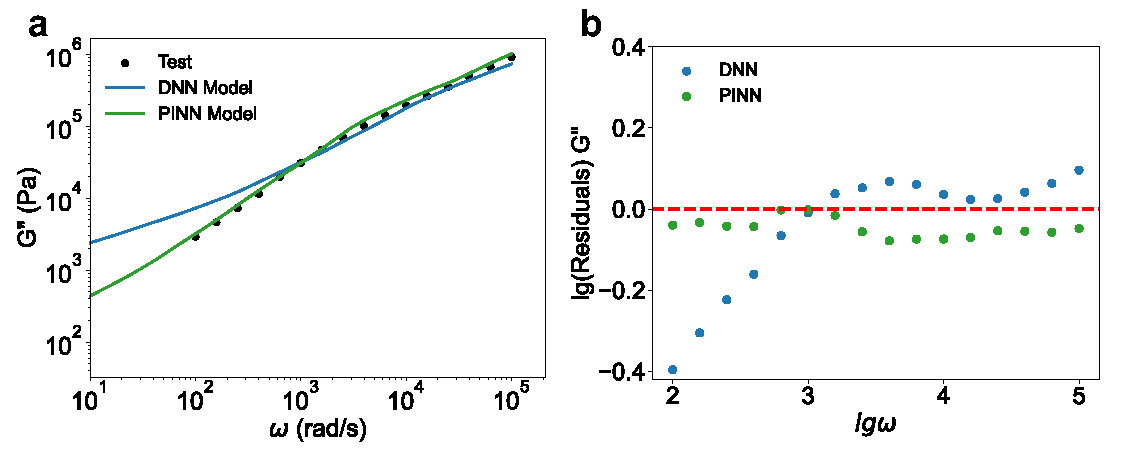
\includegraphics[width=0.8\textwidth]{Fig/pba-g2.pdf}
  \FigureBicaption{\label{pba-g2}不同分子量的PBA流体PINN和DNN建模的G"预测结果:(a)真实-预测值曲线;(b)残差图}{Prediction results of G" of PBA fluids with different DP values using PINN and DNN: (a) Real-predicted value curve; (b) Residual diagram}
\end{figure}

图\ref{pba-lossf}为tan$\delta$的预测结果,图\ref{pba-lossf}(a)为真实-预测值曲线。从真实-预测值曲线(图\ref{pba-lossf}(a))可观察到PINN建模的预测值序列与真实值分布趋势呈现更高程度的吻合,相较于传统深度神经网络(DNN)建模产生的预测曲线展现出更优的轨迹跟踪特性。进一步通过残差分布图(图\ref{pba-lossf}(b))进行评估,两种模型的预测残差虽均呈现以负偏差为主的分布特征,但PINN模型的残差绝对值显著低于DNN模型的残差绝对值,极值绝对值较小。
\begin{figure}[htbp]
  \centering
  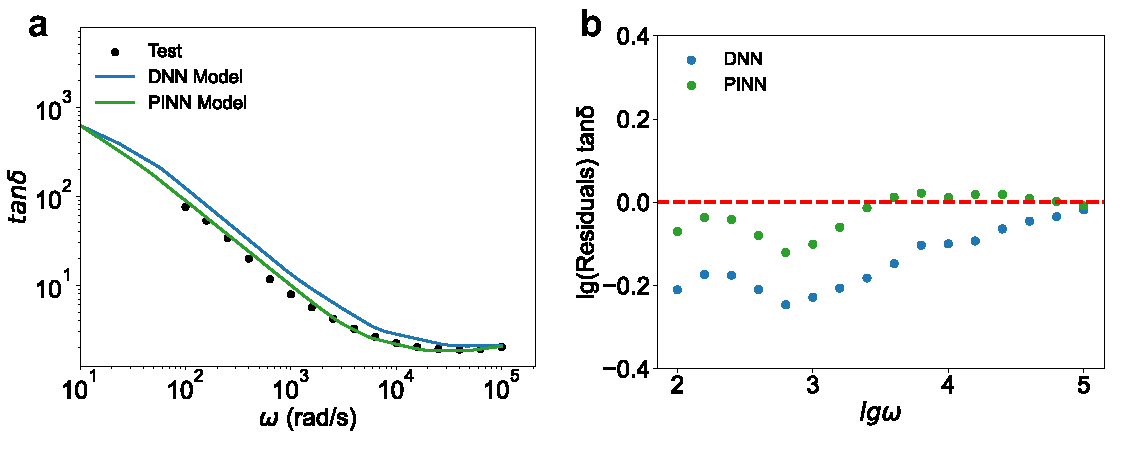
\includegraphics[width=0.8\textwidth]{Fig/pba-lossf.pdf}
  \FigureBicaption{\label{pba-lossf}不同分子量的PBA流体PINN和DNN建模的tan$\delta$预测结果:(a)真实-预测值曲线;(b)残差图}{Prediction results of tan$\delta$ of PBA fluids with different DP values using PINN and DNN: (a) Real-predicted value curve; (b) Residual diagram}
\end{figure}
\begin{figure}[htbp]
  \centering
  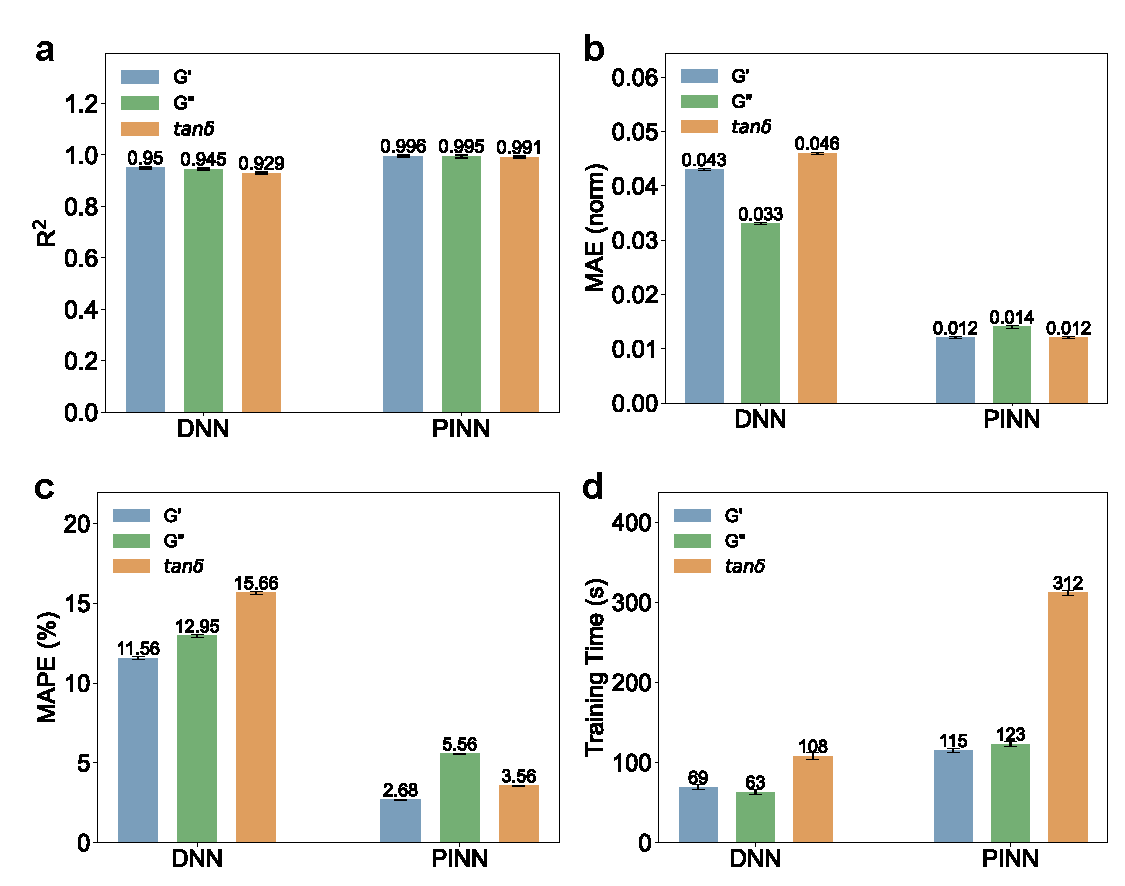
\includegraphics[width=0.8\textwidth]{Fig/pba-metrics.pdf}
  \FigureBicaption{\label{pba-metrics}不同分子量的PBA流体PINN和DNN建模的指标对比图:(a)R$^2$对比;(b)MAE对比;(c)MAPE对比;(d)训练时间对比}{Metrics comparison of PINN and DNN modeling for PBA fluids with different molecular weights: (a) R$^2$ comparison; (b) MAE comparison; (c) MAPE comparison; (d) Training time comparison}
\end{figure}
为了进一步定量分析PBA流体的模量数据PINN建模效果,本节计算测试集的R$^2$、MAE、MAPE、Training Time。图\ref{pba-metrics}为两个模型在G'预测、G"预测和tan$\delta$预测三种不同任务上的指标对比图。从图 \ref{pba-metrics} 可以看出,PINN模型在 G'、G" 和 tan$\delta$ 三个任务上的R$^2$ 均略高于 DNN 模型。此外,PINN 模型的 MAE 值在所有任务中均小于DNN模型,而 MAPE 值均小于 10\%,属于较小误差范围。相比之下,DNN模型的MAPE值均大于 10\%,表明其误差较大。这些结果表明,PINN模型在G'、G"和tan$\delta$三个任务上均具有更低的误差。然而,PINN 模型的训练时间显著更长,约为 DNN 模型的2-3倍。

这种差异表明PINN通过嵌入物理守恒方程作为正则化约束,有效抑制了DNN模型因纯数据驱动导致的过拟合现象,其残差分布的紧致性和对称性改善印证了物理先验知识对模型泛化能力的提升作用。综合可视化分析与统计指标可知,PINN框架在本研究涉及的偏微分方程反演任务中,通过融合物理机理与数据特征的双重驱动,实现了比传统数据驱动范式更优的泛化预测性能。
% PBA嵌入PFGs
\subsection{单组分PBA注入的PFGs本构建模}
本节对第二类数据,即单一分子量PBA注入制备的PFGs进行深度学习本构建模,探究在不同分子量PBA注入的PFGs上,PINN模型与DNN模型的性能对比。图\ref{pfgs-single}为两种算法模型对这类数据的预测性能对比。图\ref{pfgs-single}(a)为真实值-预测值曲线,这里对比的是tan$\delta$的预测结果。从图中可以看出,PINN模型的预测曲线与真实值曲线更为贴近,拟合效果更佳。图\ref{pfgs-single}(b)为残差图,PINN模型的残差绝对值显著低于DNN模型的残差绝对值,PINN的残差更为邻近0刻度线。综上所述,可以定性认为在此项任务中,PINN模型的泛化预测效果更佳。
\begin{figure}[htbp]
  \centering
  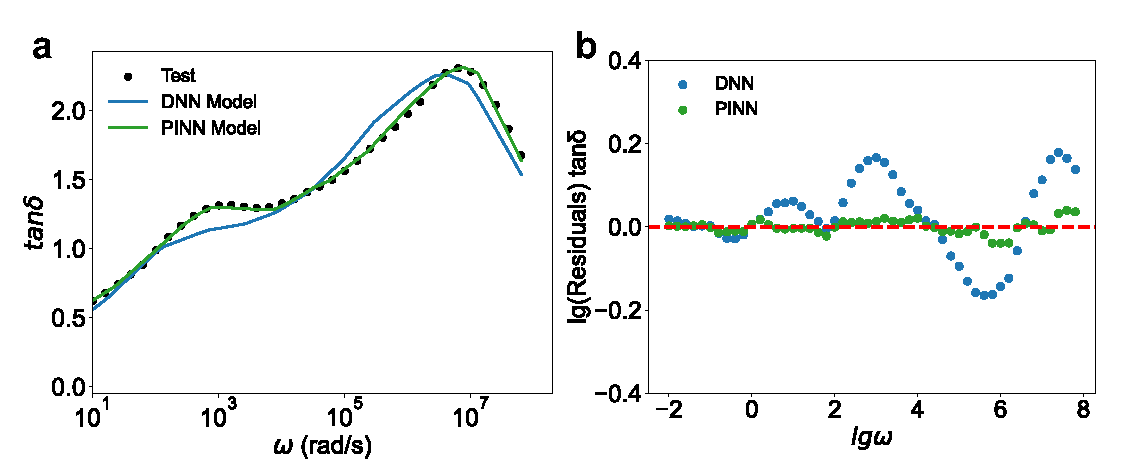
\includegraphics[width=0.8\textwidth]{Fig/pfgs-single.pdf}
  \FigureBicaption{\label{pfgs-single}单分子量PBA注入的PFGs数据PINN和DNN建模的tan$\delta$预测结果:(a)PINN和DNN在测试集上的预测值与真实值对比曲线;(b)PINN和DNN在测试集上的预测值残差图}{Prediction results of tan$\delta$ of PFGs prepared by single molecular weight PBA injection using PINN and DNN modeling: (a) Comparison curves of predicted vs. true values for PINN and DNN on test set; (b) Residual plots of predicted values for PINN and DNN on test set}
\end{figure}
为了进一步定量分析单组分PBA注入的PFGs数据的PINN建模效果,本节计算测试集的R$^2$、MAE、MAPE、Training Time。图\ref{pfgs-single-metrics}为两个模型tan$\delta$预测的指标对比图。从图中可以看出,PINN模型在该任务上的R$^2$略低于DNN模型。在MAE指标上,PINN为0.012,DNN为0.071,PINN的MAE值相比DNN降低了83.38\%。MAPE指标方面,PINN为0.03\%,DNN为8.59\%,相差近3个数量级别。这里PINN模型的R$^2$值意外地低可能是因为PINN引入的物理约束可能降低了模型对训练数据的过拟合程度,但模型的泛化能力和实际预测精度(MAPE)更好这些结果表明,PINN模型在预测单组分PBA注入的PFGs流变性能时具有更高的准确性和稳定性。然而,与前文类似,PINN模型的训练时间显著长于DNN模型,大约是后者的5倍,这是由于物理约束的引入增加了计算复杂度。
\begin{figure}[htbp]
  \centering
  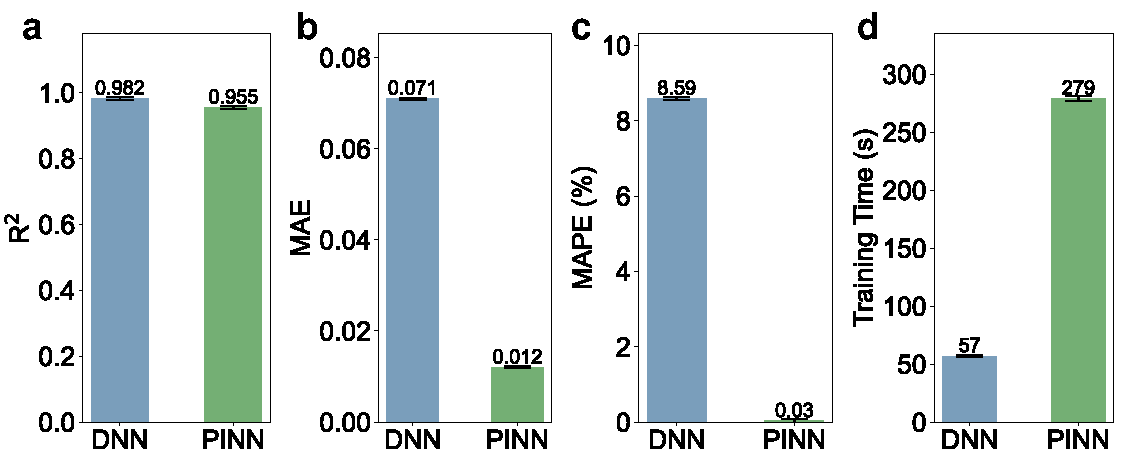
\includegraphics[width=0.8\textwidth]{Fig/pfgs-single-metrics.pdf}
  \FigureBicaption{\label{pfgs-single-metrics}单分子量PBA注入的PFGs数据PINN和DNN建模的tan$\delta$预测指标对比图:(a)R$^2$对比;(b)MAE对比;(c)MAPE对比;(d)训练时间对比}{Comparison of R$^2$, MAE, MAPE, and Training Time metrics of PINN and DNN for tan$\delta$ prediction of PFGs prepared by single molecular weight PBA injection: (a) R$^2$ comparison; (b) MAE comparison; (c) MAPE comparison; (d) Training Time comparison}
\end{figure}
综上所述,PINN模型在单组分PBA注入的PFGs数据的建模预测中展现出显著优势。从定性分析角度来看,PINN模型生成的预测曲线与实验数据点更为贴合,残差分布更加集中且接近零值。从定量分析的角度来看,尽管PINN的R²指标略低于DNN模型,但在MAE和MAPE这两个更能反映实际预测精度的指标上,PINN模型都取得了显著优势。特别是在MAPE指标上,PINN与DNN指标差近3个数量级。这表明PINN通过引入物理约束,有效抑制了过拟合现象,提高了模型的泛化能力和预测准确性。然而需要注意的是,由于引入物理约束增加了计算复杂度,PINN模型的训练时间约为DNN模型的5倍,这是可以预见的成本增加。
\subsection{多组分PBA注入的PFGs本构建模}
上一节研究了单组分PBA注入的PFGs数据建模,验证了PINN模型在处理简单制备参数特征(单一分子量)时,通过引入物理约束能够有效提升模型的泛化能力。本节将进一步探讨PINN模型在多组分PBA注入的PFGs数据上的表现,研究其在处理复杂制备参数特征(多分子量组合)时的泛化性能,以期为实际应用提供更有价值的参考。
\begin{figure}[htbp]
  \centering
  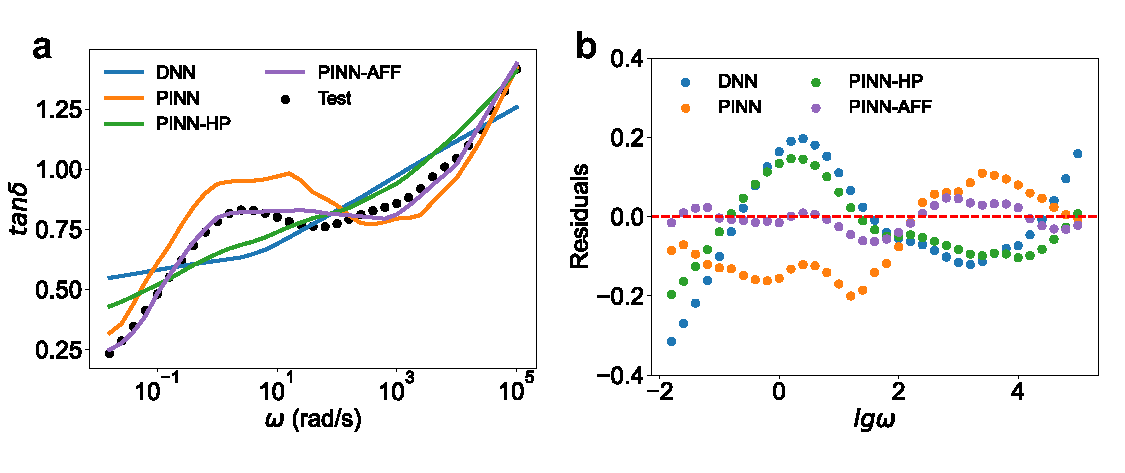
\includegraphics[width=0.8\textwidth]{Fig/pfgs-com.pdf}
  \FigureBicaption{\label{pfgs-com}多组分PBA注入制备的PFGs数据不同算法建模的tan$\delta$预测结果:(a)不同算法在测试集上的预测值与真实值对比曲线;(b)不同算法在测试集上的预测值残差图}{Prediction results of tan$\delta$ of PFGs prepared by multiple molecular weight PBA injection using different algorithms: (a) Comparison curves of predicted vs. true values on test set; (b) Residual plots of predicted values on test set}
\end{figure}
图\ref{pfgs-com}为多组分PBA注入的PFGs数据建模结果,图\ref{pfgs-com}(a)为真实值-预测值曲线,图\ref{pfgs-com}(b)为残差图。本项预测建模任务一共使用4组不同的算法建模,分别是普通DNN、普通PINN、采用哈达玛积特征融合的PINN(PINN-HP)和采用注意力特征融合的PINN(PINN-AFF)。图\ref{pfgs-com}显示PINN-AFF的预测效果最佳,预测曲线与真实值曲线最为贴近,残差分布最为集中且接近0刻度线。而其他算法模型的预测存在不同类型的偏差。

\begin{figure}[htbp]
  \centering
  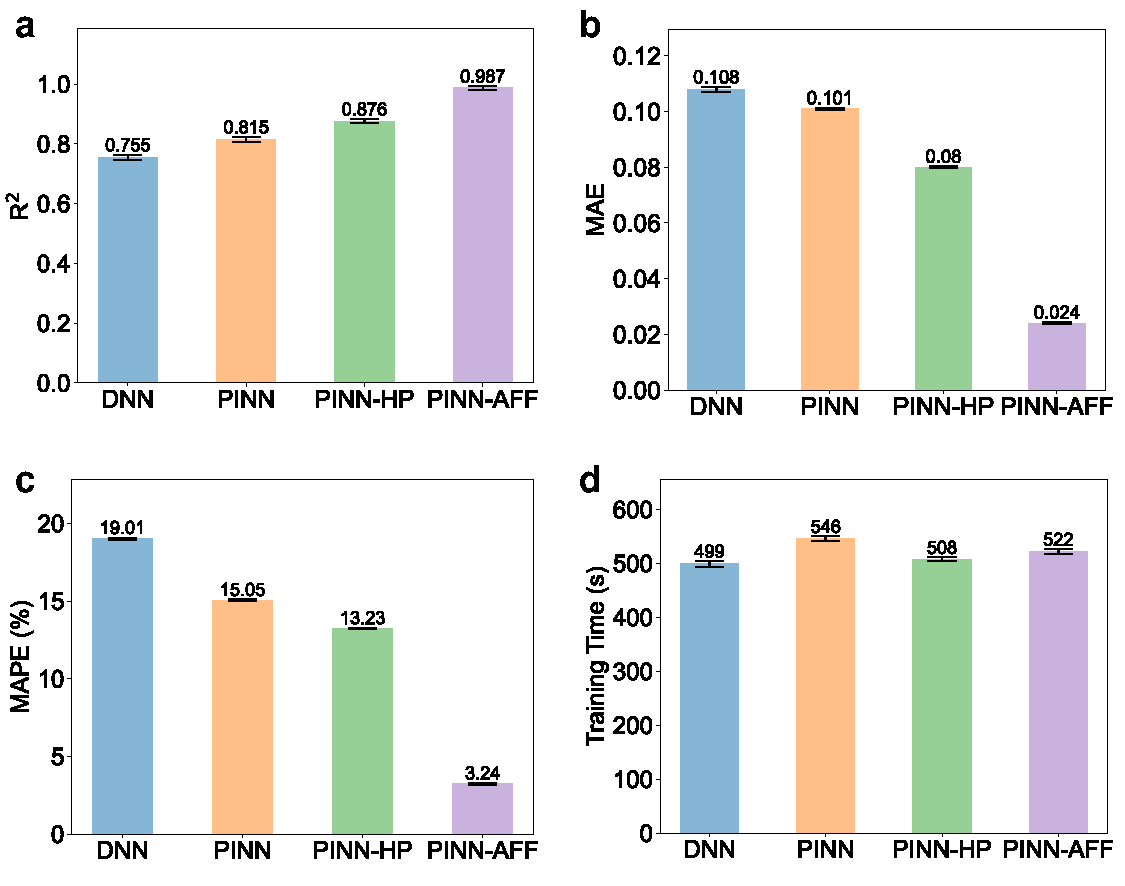
\includegraphics[width=0.8\textwidth]{Fig/pfgs-com-metrics.pdf}
  \FigureBicaption{\label{pfgs-com-metrics}多组分PBA注入制备的PFGs数据不同算法建模的tan$\delta$预测指标对比图:(a)R$^2$对比;(b)MAE对比;(c)MAPE对比;(d)训练时间对比}{Comparison of R$^2$, MAE, MAPE, and Training Time metrics of PINN and DNN for tan$\delta$ prediction of PFGs prepared by multiple molecular weight PBA injection: (a) R$^2$ comparison; (b) MAE comparison; (c) MAPE comparison; (d) Training Time comparison}
\end{figure}
为了进一步定量分析多组分PBA注入的PFGs数据的PINN建模效果,本节计算了测试集的R$^2$、MAE、MAPE和训练时间等评价指标。图\ref{pfgs-com-metrics}展示了4种不同算法模型在tan$\delta$预测任务上的性能对比。从图中可以看出,在所有评价指标上,注意力特征融合的PINN(PINN-AFF)模型均表现最佳,其次是哈达玛积特征融合的PINN(PINN-HP)模型,再次是普通PINN模型,而传统DNN模型的表现最差。这一结果表明,引入特征融合机制能够有效提升PINN模型的预测性能,其中基于注意力机制的特征融合方案尤为有效。从时间指标上看,PINN的训练时间略大于DNN,这与之前的实验一致,PINN-HP的训练时间略小于PINN,这是因为PINN-HP通过将分子量和组分含量特征融合减少了总的特征数量,减少了训练参数的数量。PINN-AFF的训练时间又略大于PINN-HP,这是因为PINN-AFF引入了注意力机制,增加了计算复杂度。


综合图\ref{pfgs-com}和图\ref{pfgs-com-metrics}的分析结果可以看出,在处理特征数量较多且特征之间存在复杂物理关系的情况下,普通PINN模型的学习泛化能力相对有限。针对这一问题,本研究提出了两种改进方案。首先,哈达玛积特征融合的PINN(PINN-HP)模型通过将分子量和组分含量特征进行哈达玛积运算进行特征融合,这种方式相当于为模型预设了特征之间的物理关联,从而提升了模型的预测效果。在此基础上,注意力特征融合的PINN(PINN-AFF)模型进一步引入了注意力机制,对不同分子量与组分含量融合后的联合特征进行注意力加权。这种机制能够有效学习不同高分子链段之间的相互作用关系,通过注意力分数定量描述组分间的流变学相互作用强度,并能自动识别关键组分的影响程度,例如能够捕捉到高分子量组分对整体流变学性能的主导作用。实验结果表明,这两种改进方案都显著提升了模型性能,其中PINN-AFF模型取得了最优的预测效果。

% CVAE组分预测
\subsection{CVAE组分预测的多模态解分析}
\begin{figure}[htbp]
  \centering
  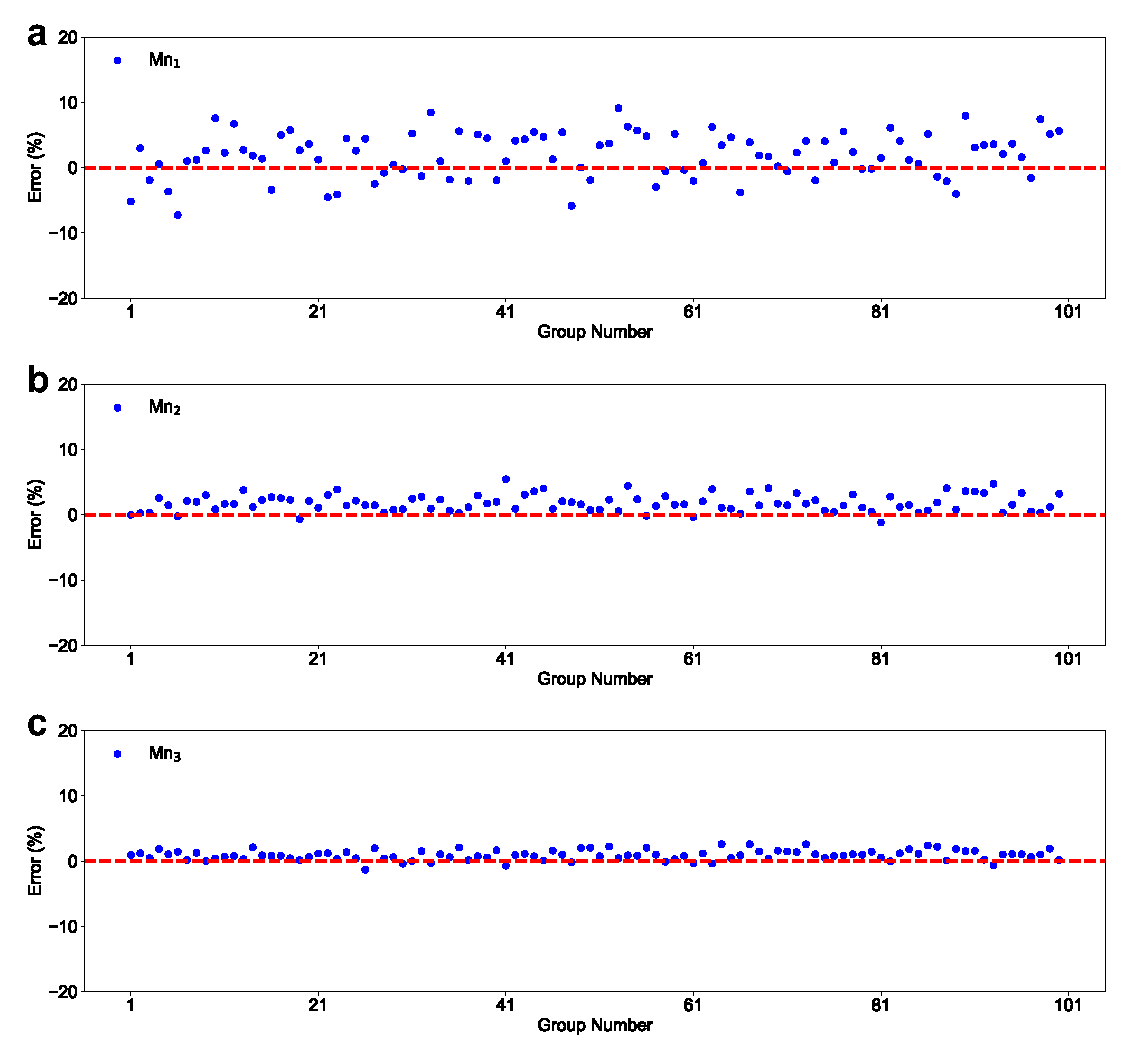
\includegraphics[width=0.8\textwidth]{Fig/reverse-redisual-Mn.pdf}
  \FigureBicaption{\label{reverse-redisual-Mn}CVAE生成的100组多模态解中不同分子量组分Mn$_1$、Mn$_2$、Mn$_3$的残差分布:(a)Mn$_1$残差分布;(b)Mn$_2$残差分布;(c)Mn$_3$残差分布}{Residual distributions of 100 multimodal solutions generated by CVAE for different molecular weight components Mn$_1$, Mn$_2$, Mn$_3$: (a) Residual distribution of Mn$_1$; (b) Residual distribution of Mn$_2$; (c) Residual distribution of Mn$_3$}
\end{figure}

\begin{figure}[htbp]
  \centering
  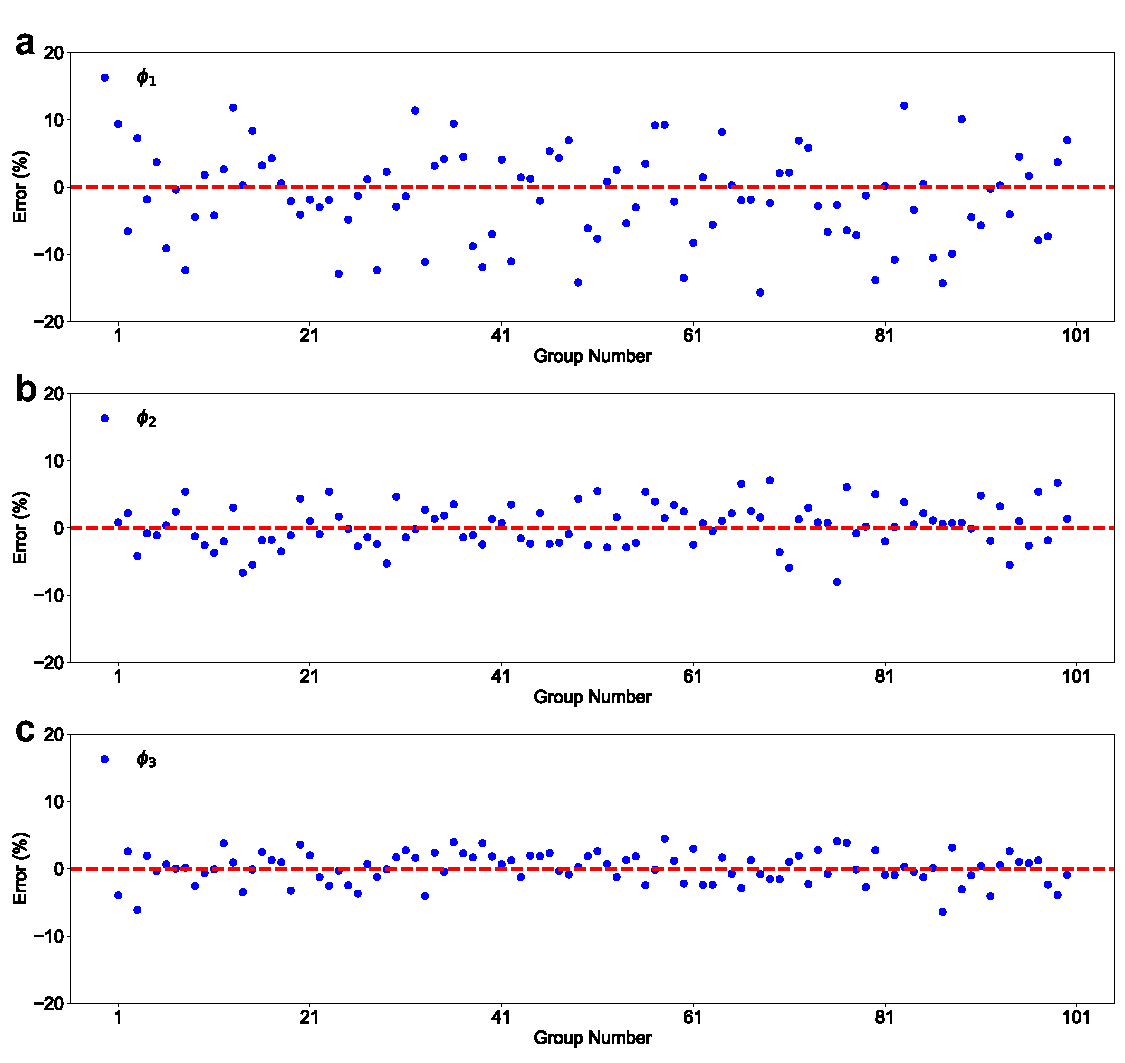
\includegraphics[width=0.8\textwidth]{Fig/reverse-redisual-phi.pdf}
  \FigureBicaption{\label{reverse-redisual-phi}CVAE生成的100组多模态解中不同组分含量$\phi_1$、$\phi_2$、$\phi_3$的残差分布:(a)$\phi_1$残差分布;(b)$\phi_2$残差分布;(c)$\phi_3$残差分布}{Residual distributions of 100 multimodal solutions generated by CVAE for different component contents $\phi_1$, $\phi_2$, $\phi_3$: (a) Residual distribution of $\phi_1$; (b) Residual distribution of $\phi_2$; (c) Residual distribution of $\phi_3$}
\end{figure}
本节探索了使用CVAE模型从材料的流变学性质反向预测其组分配比的可行性。基于训练完成的生成模型,我们输入目标流变学参数[$\omega$,G',G",tan$\delta$],生成100组多模态解,并对生成结果进行系统的残差分析。

图\ref{reverse-redisual-Mn}展示了分子量参数Mn的残差分布。结果表明,三种分子量组分Mn$_1$、Mn$_2$、Mn$_3$的残差均呈现正态分布特征,最大偏差约为10\%,处于可接受范围内。残差大小依次为Mn$_1$>Mn$_2$>Mn$_3$。图\ref{reverse-redisual-phi}则显示了组分含量参数$\phi$的残差分布。$\phi_1$、$\phi_2$、$\phi_3$同样呈现正态分布特征,最大偏差约为20\%,残差大小顺序为$\phi_1$>$\phi_2$>$\phi_3$。

值得注意的是,在测试集中Mn$_1$<Mn$_2$<Mn$_3$,$\phi_1$<$\phi_2$<$\phi_3$,由此观察到残差大小与参数实际值呈现负相关关系 - 即参数绝对值越小,其预测误差反而越大。这一现象揭示了模型在预测较小数值参数时的精度局限性,实际应用时,可以通过调整量纲一定程度缓解这一问题。
\begin{figure}[htbp]
  \centering
  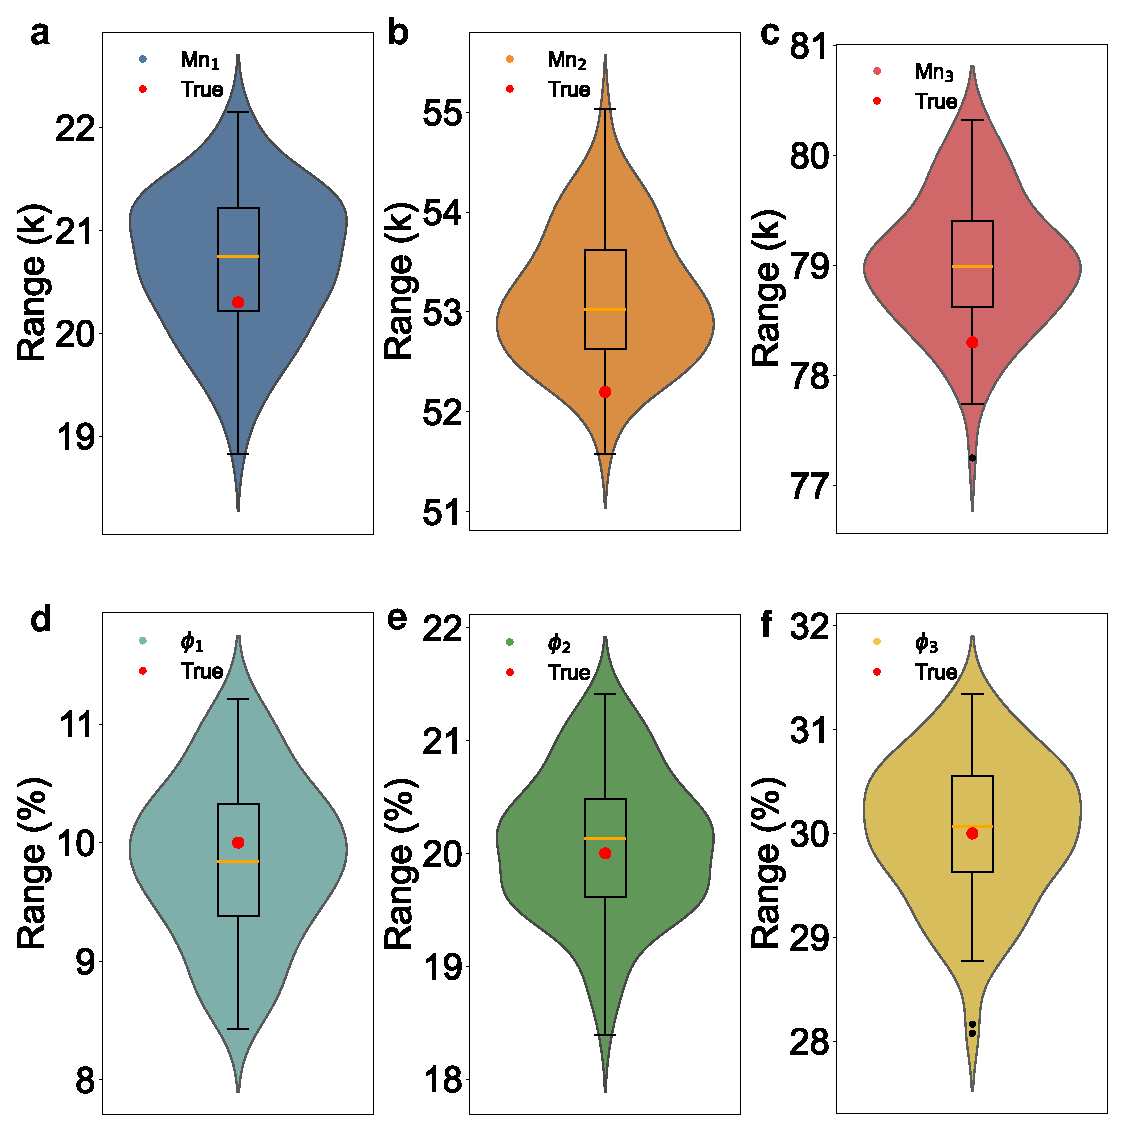
\includegraphics[width=0.8\textwidth]{Fig/reverse-violin.pdf}
  \FigureBicaption{\label{reverse-violin}CVAE生成的100组多模态解的violin图:(a)分子量参数Mn$_1$的多模态解分布;(b)分子量参数Mn$_2$的多模态解分布;(c)分子量参数Mn$_3$的多模态解分布;(d)组分含量参数$\phi_1$的多模态解分布;(e)组分含量参数$\phi_2$的多模态解分布;(f)组分含量参数$\phi_3$的多模态解分布}{Violin plots of 100 multimodal solutions generated by CVAE: (a) Distribution of multimodal solutions for molecular weight parameter Mn$_1$; (b) Distribution of multimodal solutions for molecular weight parameter Mn$_2$; (c) Distribution of multimodal solutions for molecular weight parameter Mn$_3$; (d) Distribution of multimodal solutions for component content parameter $\phi_1$; (e) Distribution of multimodal solutions for component content parameter $\phi_2$; (f) Distribution of multimodal solutions for component content parameter $\phi_3$}
\end{figure}

图\ref{reverse-violin}为生成数据的violin图。(a-f)分别展示了分子量参数Mn$_1$、Mn$_2$、Mn$_3$和组分含量参数$\phi_1$、$\phi_2$、$\phi_3$的多模态解分布情况。由图可见,真实分子量数据(Mn)在生成分子量数据的下四分位数附近,总体生成偏大,大部分数据分布在中位数附近,真实组分含量数据($\phi$)在生成组分含量数据中位数附近,总体生成效果良好。从核密度曲线的形态来看,所有参数的分布均呈现出中间宽、两端窄的典型小提琴形状,表明数据分布较为集中。整体数据分布服从正态分布,无明显多峰值特征。具体分析各参数的核密度曲线最宽处(即数据最集中处)与中位数线的相对位置:Mn$_1$的核密度曲线最宽处位于中位数线上方,表明生成数据相对真实值略有高估;Mn$_2$的核密度曲线最宽处位于中位数线下方,显示生成数据略低于中位数水平;而其余各参数(Mn$_3$、$\phi_1$、$\phi_2$、$\phi_3$)的核密度曲线最宽处与中位数线基本重合,说明这些参数的生成分布更为准确。异常点分析结果显示,所有参数的异常点数量均较少,表明生成数据整体质量较高。
\begin{figure}[htbp]
  \centering
  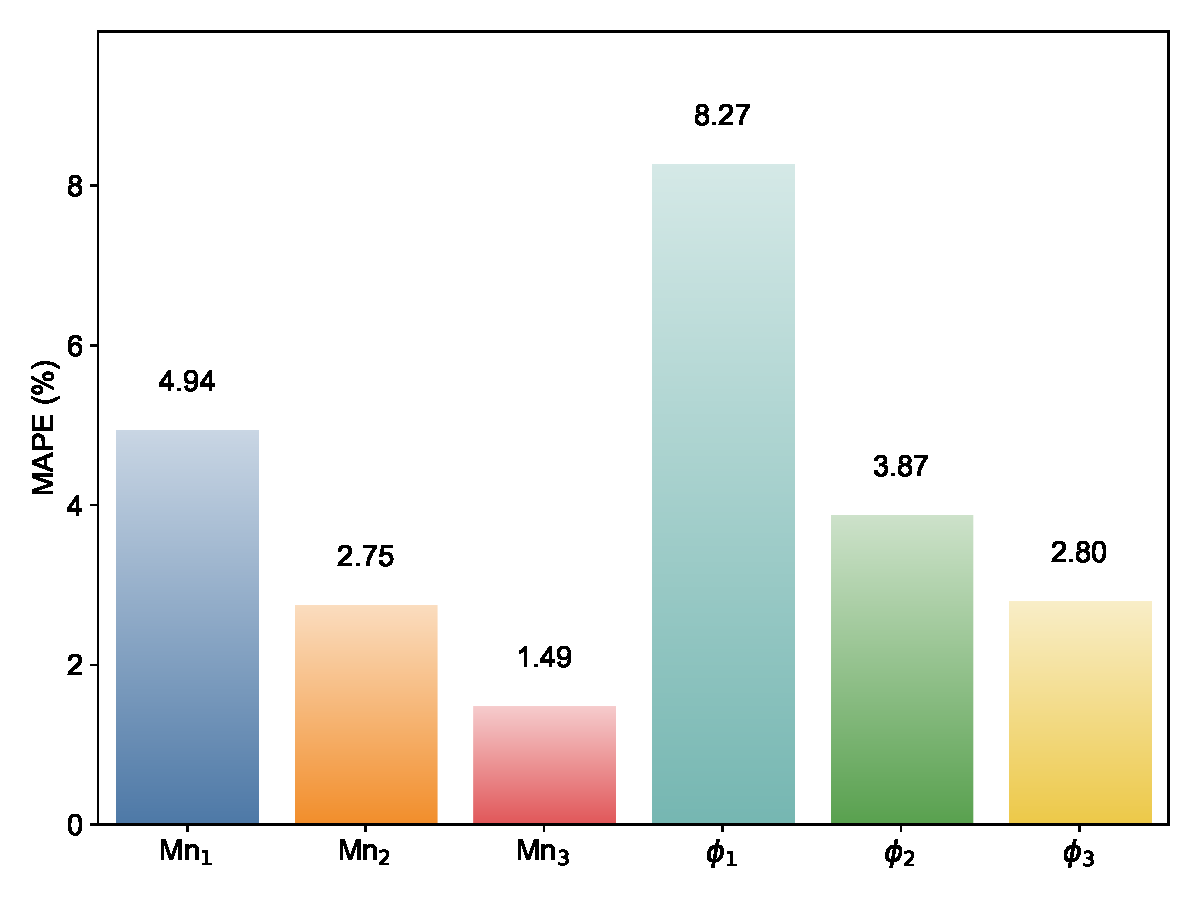
\includegraphics[width=0.8\textwidth]{Fig/MAPE_bar_chart.pdf}
  \FigureBicaption{\label{reverse-mape}CVAE生成的100组多模态解中分子量参数Mn$_1$、Mn$_2$、Mn$_3$和组分含量参数$\phi_1$、$\phi_2$、$\phi_3$的MAPE图}{MAPE chart of molecular weight parameters Mn$_1$, Mn$_2$, Mn$_3$ and component content parameters $\phi_1$, $\phi_2$, $\phi_3$ of 100 multimodal solutions generated by CVAE}
\end{figure}

图\ref{reverse-mape}为MAPE的条形图。从图中可以看出,分子量参数Mn$_1$、Mn$_2$、Mn$_3$的MAPE值分别为4.94\%、2.75\%、1.49\%,组分含量参数$\phi_1$、$\phi_2$、$\phi_3$的MAPE值分别为8.27\%、3.87\%、2.80\%。这些数据揭示了几个重要的趋势:首先,分子量参数的预测总体优于组分含量参数,这表明模型在预测分子量特征时具有更好的准确性;其次,无论是分子量还是组分含量参数,都呈现出随着数值增大(即Mn$_1$ < Mn$_2$ < Mn$_3$和$\phi_1$ < $\phi_2$ < $\phi_3$)预测误差逐渐减小的规律,这与之前残差分析的结果相一致。特别值得注意的是,即使是预测误差最大的$\phi_1$,其MAPE值也仅为8.27\%,而其他参数的MAPE值都控制在5\%以内,这说明模型整体的预测精度达到了较高水平,具有良好的实用价值。

综合以上分析结果,CVAE模型在从流变学性质反向预测组分配比的任务中展现出了良好的性能。通过残差分析、violin图分析和MAPE定量分析,我们可以得出以下主要结论:首先,模型生成的组分配比数据整体呈现正态分布特征,预测结果的分布集中且稳定,异常值较少;其次,预测误差随着参数数值的增大而减小,这一特征在分子量和组分含量两类参数中均有体现。这种误差分布特征可能源于在数据标准化过程中,较小数值参数更容易受到数值舍入和归一化误差的影响。第三,从MAPE指标来看,分子量参数的预测精度普遍优于组分含量参数,但两类参数的预测误差均控制在可接受范围内(最大MAPE为8.27\%)。这些结果表明,CVAE模型能够有效地实现从材料性质到材料制备参数的反向设计,为高分子材料配方开发提供了一种可靠的数据驱动方法。

\subsection{正逆向联合建模分析}
\begin{figure}[htbp]
  \centering
  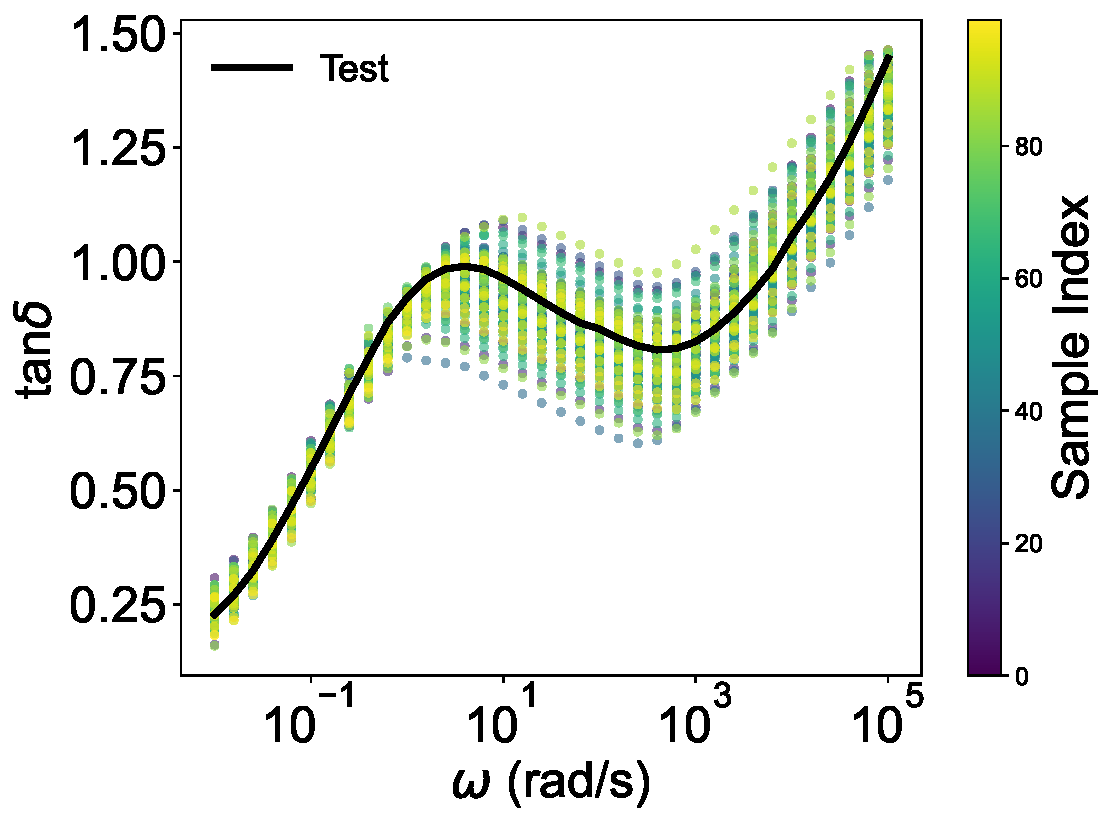
\includegraphics[width=0.8\textwidth]{Fig/prediction_results.pdf}
  \FigureBicaption{\label{cvae2pinn}100组CVAE生成的多模态解输入PINN模型后的预测值曲线}{Prediction curves of 100 multimodal solutions generated by CVAE after input into PINN model}
\end{figure}
上一节通过分析CVAE生成的100组生成组分数据与真实组分数据的误差来确定CVAE模型的生成效果,但是这种分析方法存在一定的局限性。首先,组分数据与频率-损耗角正切曲线之间存在多对一的映射关系,即理论上可能存在多种不同的组分配比,制备出来的材料具有相同或近似的频率-损耗角正切曲线。这种多解性是高分子材料设计中的一个普遍现象,源于不同分子量组分之间复杂的相互作用。其次,组分配比的微小变化可能导致材料性能的显著差异,这种非线性关系使得仅通过比较组分数据的误差来评估模型效果是不够全面的。

从实验验证的角度来看,最准确的分析方法应该是按照生成的组分配比分别制备材料样品,通过DMA频率扫描实验测试其损耗角正切,并与目标曲线进行对比。然而,考虑到实验成本和时间效率,这种方法在实际操作中并不现实。为了在保证验证可靠性的同时提高效率,本节采用了一种替代方案:将CVAE模型生成的100组组分特征输入到已训练好的PINN模型中,通过PINN的预测结果来评估CVAE生成结果的质量。这种方法虽然不能完全替代实验验证,但可以在一定程度上反映生成组分的合理性。

图\ref{cvae2pinn}展示了这100组特征输入PINN后得到的频率-损耗角正切曲线,其中Test线代表原始真实特征对应的预测曲线。从图中可以观察到,这100组预测特征绘制的曲线形成了一个连续的曲线带,且具有以下特点:首先,曲线带的整体趋势与Test线高度一致,表明生成的组分特征能够较好地捕捉材料的主要流变学特性;其次,Test线位于曲线带的中心区域,说明生成结果的分布是合理的;最后,曲线带的宽度随频率变化呈现出不均匀的特征,这反映了在不同频率区间,组分配比对材料性能的影响程度是不同的。这种曲线带的分布特征也从另一个角度验证了CVAE模型在材料组分反演任务中的有效性。

通过建立PINN-CVAE的联合建模,可以建立一个自适应增强的流变学机器学习系统。该系统的工作流程如下:首先,PINN模型通过物理约束和特征融合机制对流变学数据进行正向建模,建立组分特征到流变学性质的映射关系。在实际应用过程中,通过真实实验获得的新数据可以不断补充到训练集中,进一步提升PINN模型的预测精度。与此同时,CVAE模型负责从目标流变学性质反向生成可能的组分配比方案,为材料设计提供多样化的参考。这些由CVAE生成的组分方案可以输入到PINN模型中进行快速评估和筛选,通过比较预测曲线与目标曲线的吻合度,筛选出最具潜力的组分配比进行实验验证,从而大大减轻实验负担。最后,实验验证结果又可以作为新的训练数据反馈给两个模型,形成一个不断优化的闭环系统。这种联合建模方法充分发挥了两种模型的优势,既保证了预测的物理合理性,又提供了材料设计的多样化方案,同时通过数据驱动和实验验证的结合,实现了系统性能的持续提升。

% 本章小结 总结与展望
\section{本章小结}
本章主要围绕PINN与CVAE两类深度学习模型在高分子流变学数据建模及组分反演中的应用进行了研究。本章首先对比了传统DNN模型与基于物理先验约束的PINN模型在处理高维数据与复杂特征时的性能差异。在PINN建模中使用自适应权重机制,首先对PBA流体和单PBA注入制备的PFGs流体进行建模,结果表明PINN相比DNN具有更好的泛化预测效果。实验结果显示,普通PINN模型在一定程度上能够提高预测精度,但其泛化能力在特征数量较多且分布稀疏场景时表现一般,具体为在预测多组分PBA注入制备的PFGs流体时,模型预测效果较差。为此,本章进一步提出了两种特征融合改进方案——哈达玛积特征融合(PINN-HP)和注意力特征融合(PINN-AFF),通过预设和学习输入特征之间的物理关联,有效地改善了模型对各类复杂非线性关系的捕捉能力,从而解决特征稀疏的问题。从R$^2$、MAE、MAPE多项评价指标来看,PINN-AFF模型在预测准确性和稳定性上均明显优于传统DNN和普通PINN模型,尽管其训练时间略长,但整体优势十分明显,这为流变学数据的高精度预测提供了新思路。

在PINN模型取得显著进展的同时,本章还深入探讨了利用CVAE模型进行材料组分反演的可行性。该部分工作主要通过将目标流变学参数(如频率$\omega$、G'、G"和tan$\delta$)作为输入,生成多模态解,并对生成数据的残差分布、核密度及异常点进行了详细分析。结果表明,无论是分子量参数(Mn)还是组分含量参数($\phi$),生成数据均基本呈现正态分布特征,且随着参数数值的增大,预测误差逐步减小,MAPE指标均控制在较低水平,验证了模型在反向预测材料配方比例方面的高精度和鲁棒性。这一研究内容解决了传统回归方法单一输出的问题,而且为基于数据驱动的材料设计提供了具有多解性的参考方案,在真实的实验应用中可以使用这些多模态解来辅助调整实验设计,从而提高实验效率。

此外,本章还对各模型在训练时间和资源消耗上的表现进行了比较和分析,指出尽管理论上PINN类模型由于引入了物理约束及复杂特征融合模块而导致训练时间较长,但其在捕捉复杂物理特性和有效泛化方面的优势足以弥补这一不足。同时,通过对比分析,可以发现深度学习模型在处理小数值参数时仍存在归一化误差,未来可通过调整量纲转换和数据预处理进一步优化模型效果。

最后,本章设计了PINN-CVAE联合建模方法,通过将PINN的正向预测能力与CVAE的反向生成能力相结合,构建了一个自适应增强的流变学机器学习系统。该系统利用PINN模型进行正向建模,通过物理约束和特征融合机制建立组分特征到流变学性质的映射关系;同时利用CVAE模型进行反向生成,从目标流变学性质生成多种可能的组分配比方案。两个模型相互配合,形成闭环优化系统:CVAE生成的组分方案可通过PINN快速评估筛选,实验验证结果又可作为新数据反馈给模型进行训练。这种联合建模方法既保证了预测的物理合理性,又提供了材料设计的多样化方案,为高分子材料的智能设计提供了新思路。

综合来看,本章对PINN系列模型和CVAE模型进行了初步构建、改进与验证,展示了深度学习在流变学数据预测和材料组分反演中的应用潜力。虽然目前的结果仍存在不足,但实验数据为后续高分子材料设计和流变特性模拟提供了一定的理论依据和参考。总体而言,本章工作初步验证了结合物理信息与深度学习方法的思路,并为未来进一步改进材料配方设计提出了一些启示。
